% !TEX root = ../main.tex
%
\chapter{User Interface Design}
\label{sec:design}

This chapter outlines the design of the prototype, focusing in the user interface and the user experience. The design process was informed by the initial user research.

\section{User Flow and Navigation}
\label{sec:design:flow}

As an initial step in the design process, a user flow diagram was created to visualize required user interaction and their relations. 
In a first rough sketch, key interactions were arranged in a linear sequence, representing the typical workflow when creating NeRF models (\ref{fig:design:flow-1}).

\begin{figure}[htb]
	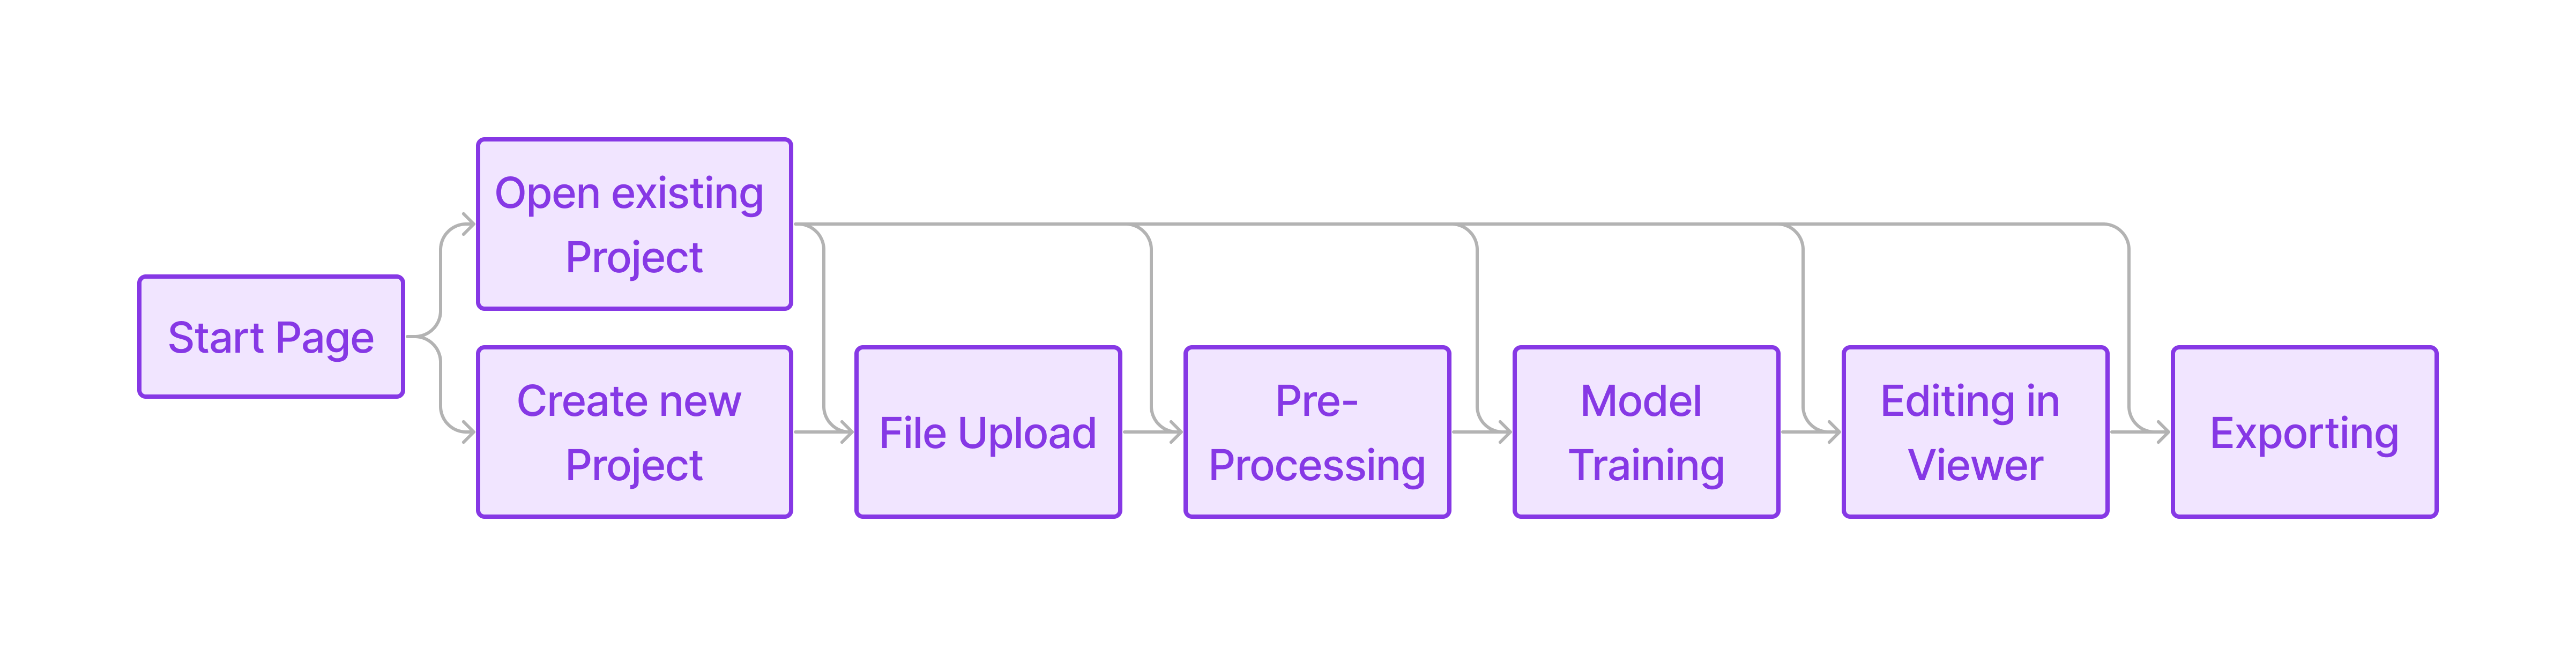
\includegraphics[width=\textwidth]{figures/flow-1.png}
	\caption{Flow Diagram}
	\label{fig:design:flow-1}
\end{figure}

Building on this outline, complex interaction were broken down into smaller steps to scope out what user actions were required to complete a task.
Interactions could then be group into views, and the navigation between these views could defined.
The views were also enriched with more detailed information on the exact user interactions (\ref{fig:design:flow-2}).

\begin{figure}[htb]
  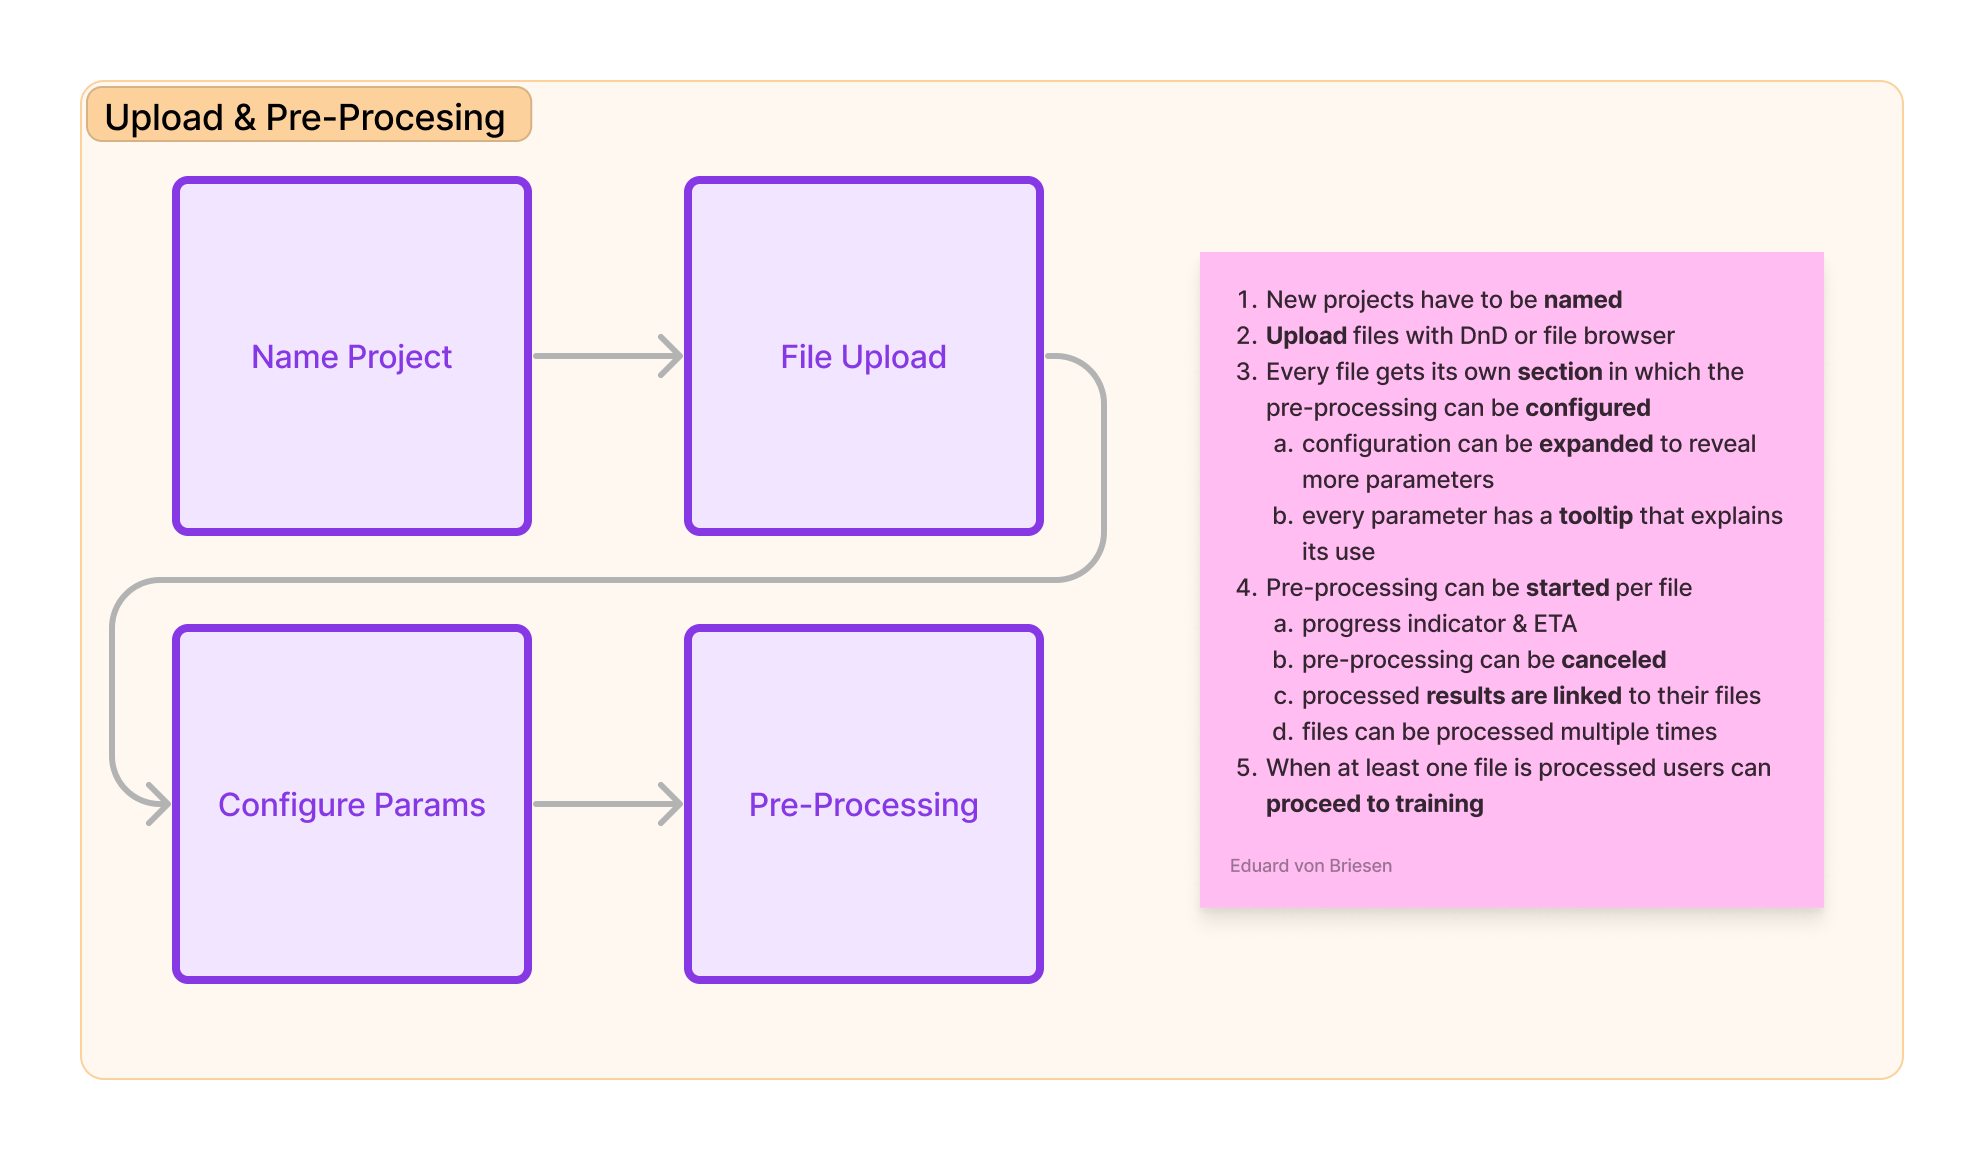
\includegraphics[width=\textwidth]{figures/flow-2.png}
  \caption{Excerpt of a View from the Flow Diagram with detailed interactions}
  \label{fig:design:flow-2}
\end{figure}

These diagrams were used as a reference throughout the design and development process, to ensure a structure that followed the user's mental model and to keep the user interface consistent.

\section{User Interface}

The user interface was designed to be as simple as possible, while still providing all necessary functionality. 
The design of the prototype can be broken down into two main parts: a dashboard that gives an overview of all projects and a project section that provides users with the tools to create and edit NeRF models.

\subsection{Dashboard}

The dashboard is the first view that users see when opening the application. It shows all previously created projects and allows users to create new ones. 
Projects are represented as cards, showing the project name, a preview of on the provided input images (if present), and tags the indicate the current status of the project.
An additional card is present through which users can create a new project, by providing a name.
Projects can be opened by clicking a button on the respective card, when creating a new project, users are redirected to the project section.

\begin{figure}[htb]
  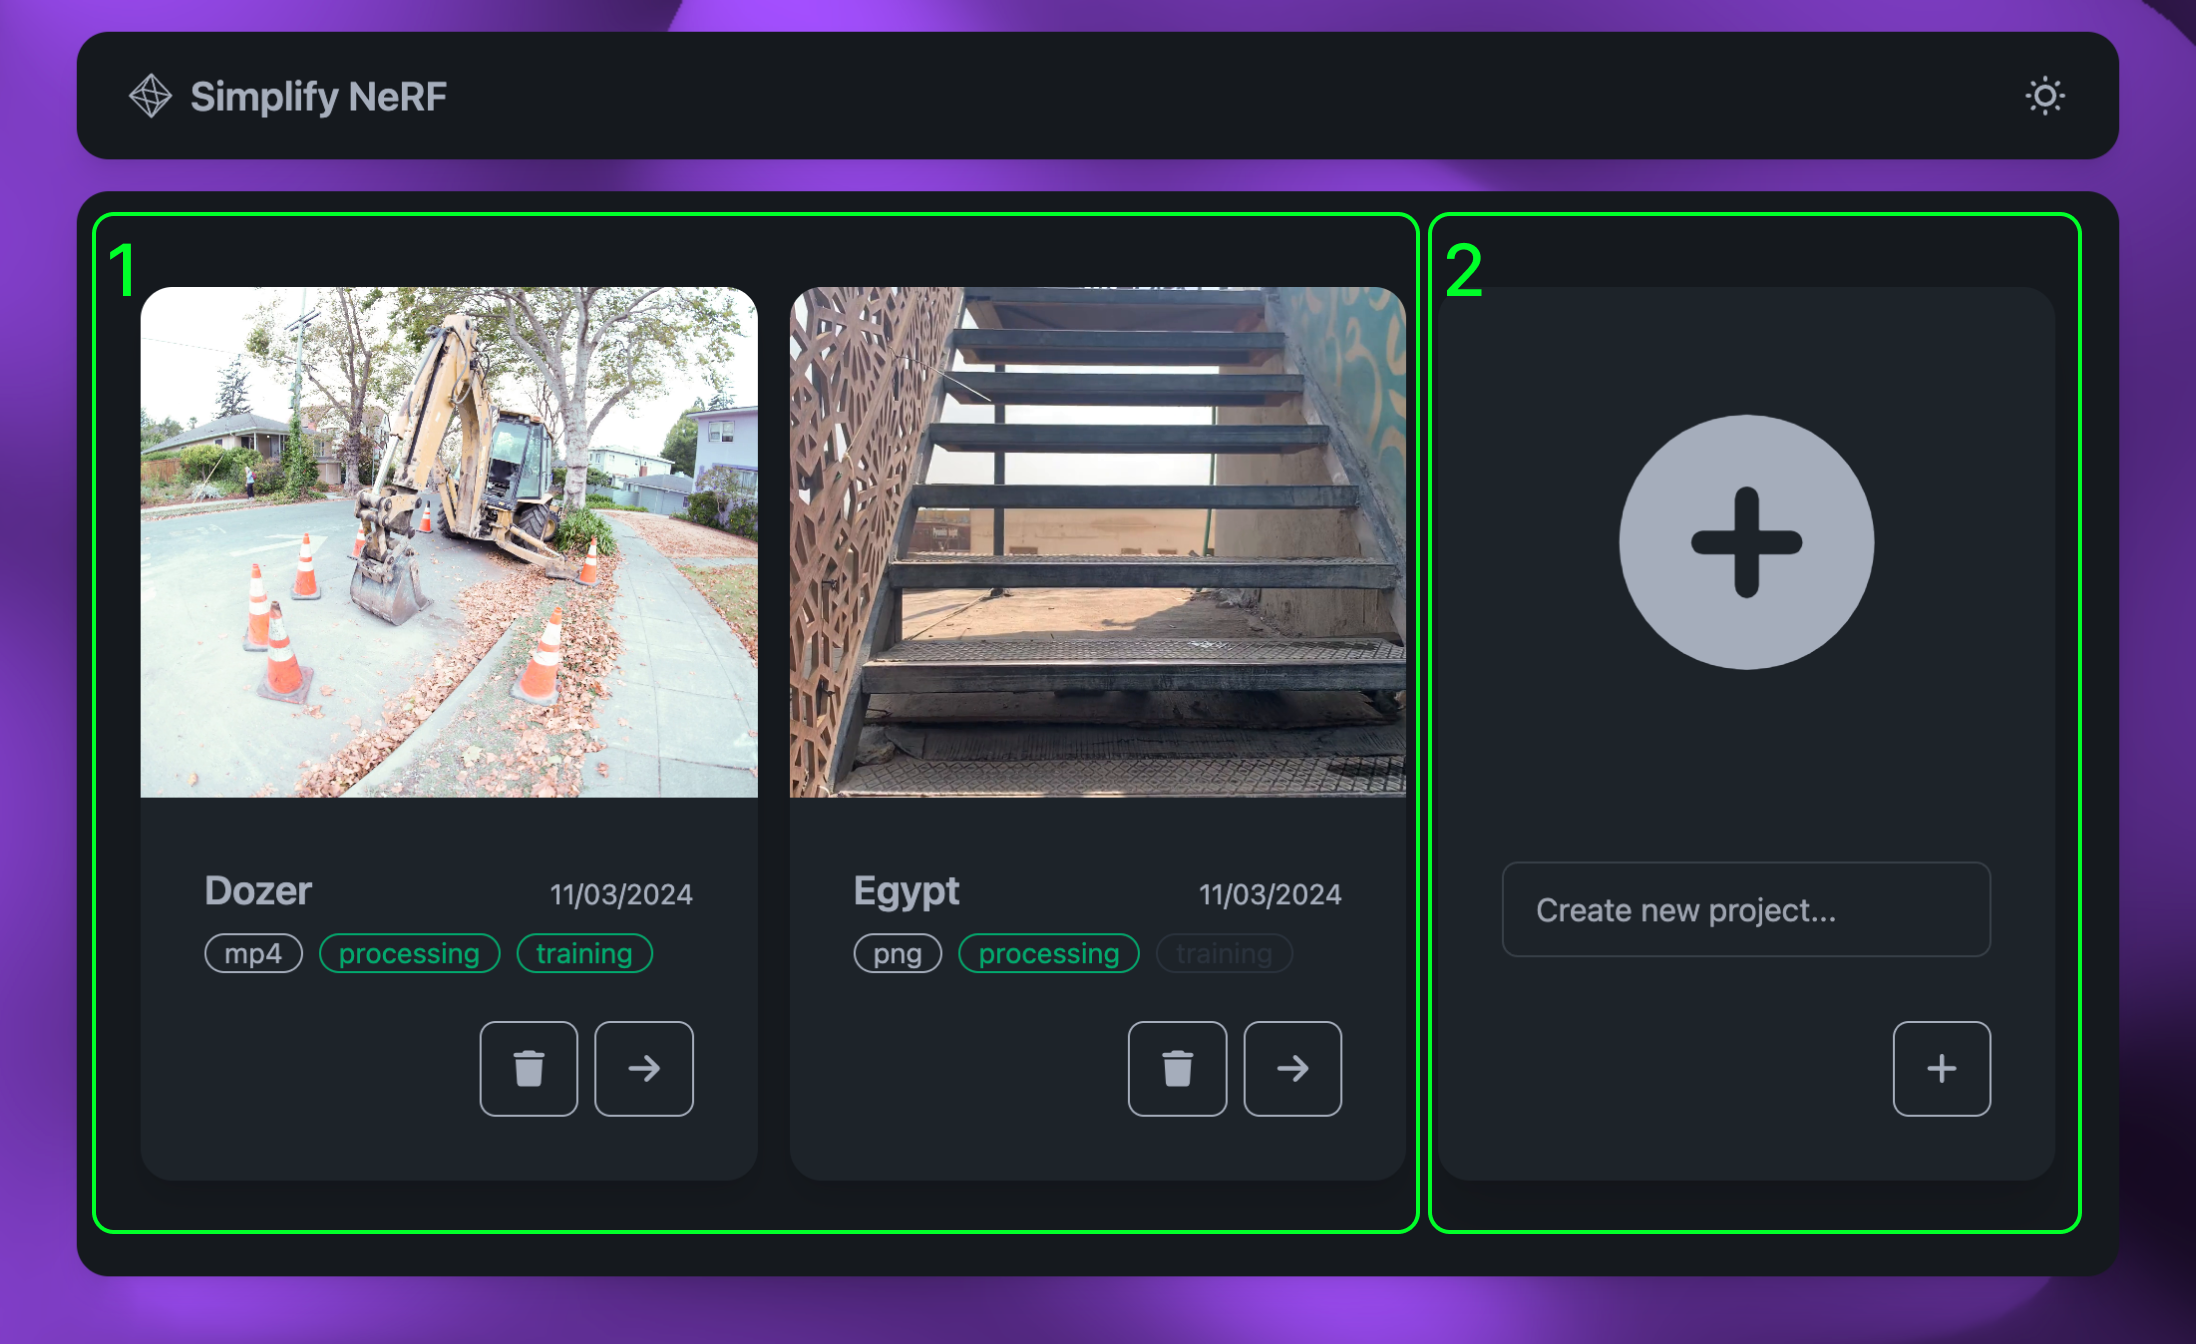
\includegraphics[width=\textwidth]{figures/view-overview.png}
  \caption{Dashboard}
  \label{fig:design:dashboard}
\end{figure}

\subsection{Project Section}

The project section is the core of the application, through which users can create and edit NeRF models.
The section is divided into three parts: the input section, the training section, and the rendering section.
Across all sections, users user can track there progress through a progress bar at the top of the screen, that also enables easy navigation between the different sections.

\subsubsection{Input Section}

The input section combines the first few interactions, as mapped out in the user flow diagram.
First users are prompted to upload there input data, which can be done by dragging and dropping files into the browser window or by clicking a button to open a file dialog.
Files can be either a set of images or a video, and there are some guardrails in place to ensure that the input data is valid.
Once the input data is uploaded, it has to be processed before it can be used for training. 
The pre-processing can be configured by the user, this includes parameters such as the lense-type, or matching method.
Parameter input fields vary based on the type of input data, and are only shown when relevant.
Once the user is satisfied with the settings, they can start the pre-processing.
Feedback on the progress of the pre-processing is given through a console that shows the output of the process running on the server.
When the pre-processing is finished, the user can move on to the training section. 

\begin{figure}[htb]
  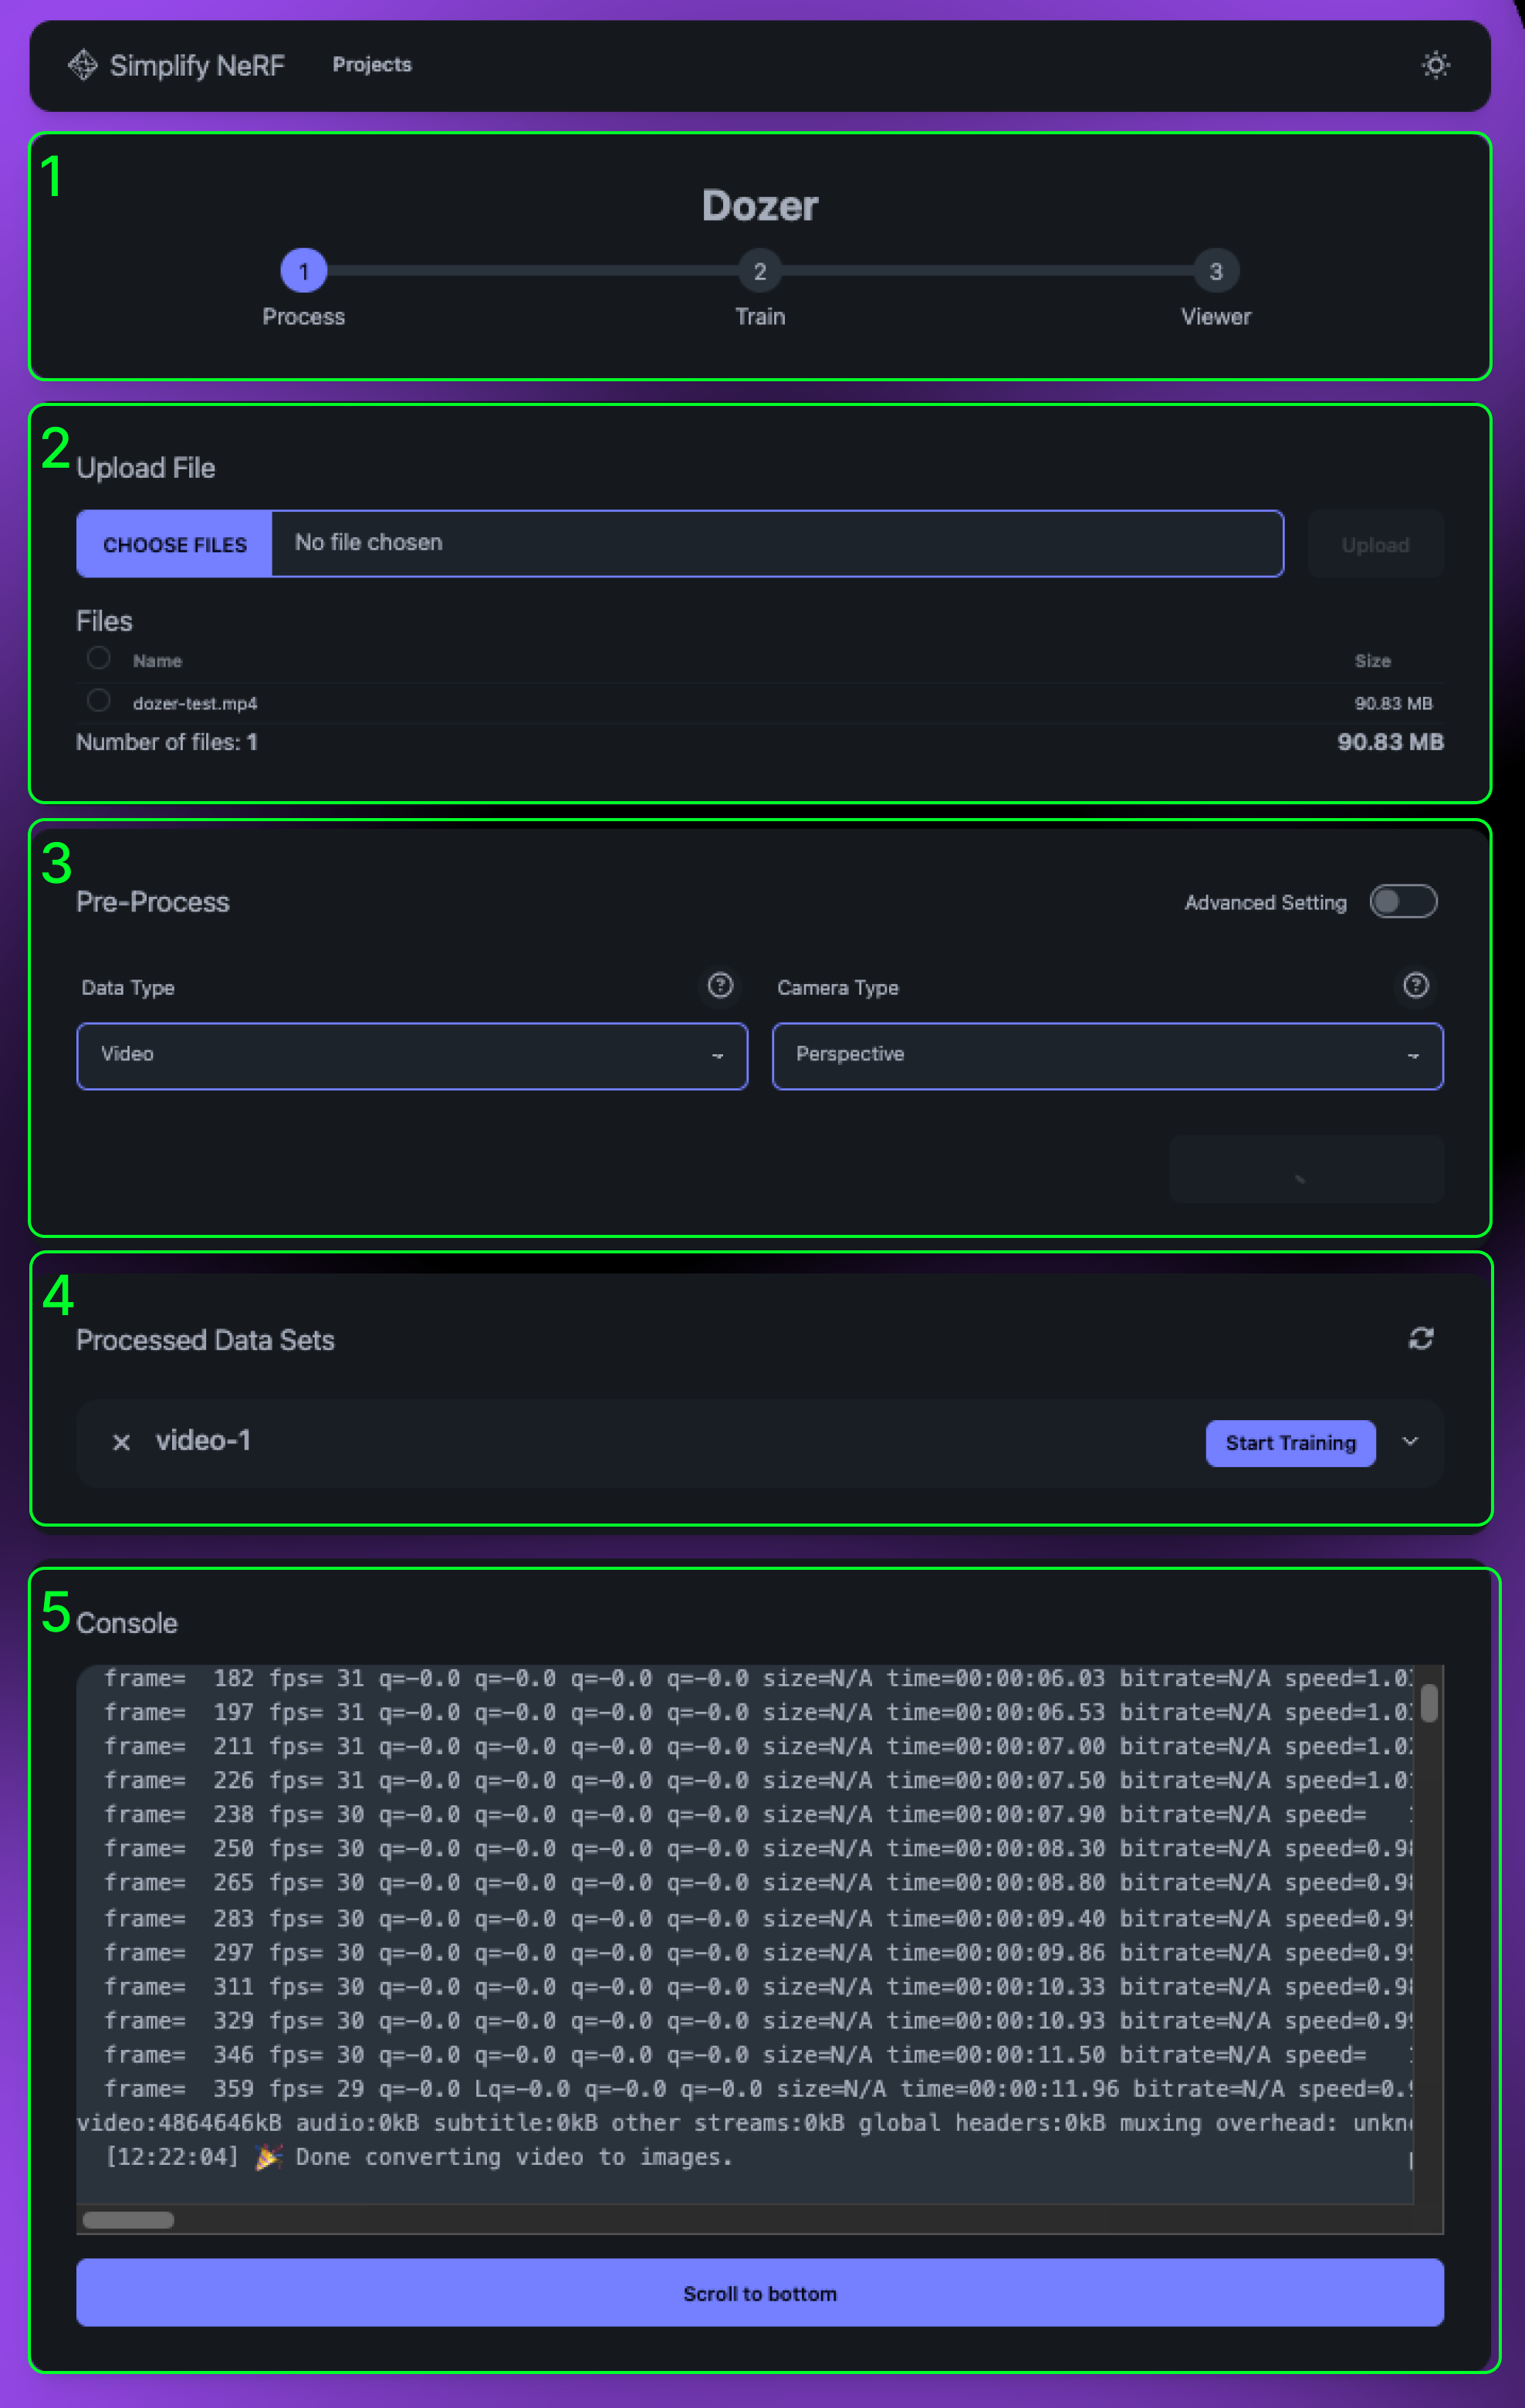
\includegraphics[width=\textwidth]{figures/view-process.png}
  \caption{Processing Input Data}
  \label{fig:design:input-section}
\end{figure}

In case the data was already pre-processed, a list ist visible that shows all available pre-processed data, and the user can select one to use for training.
Users can also inspect the configuration with which the data was pre-processed, and delete it if necessary.

\subsubsection{Training Section}

The training section is structured similarly to the input section, with a form that allows users to configure the training process, and a console that shows the output of the training process running on the server.

\begin{figure}[htb]
  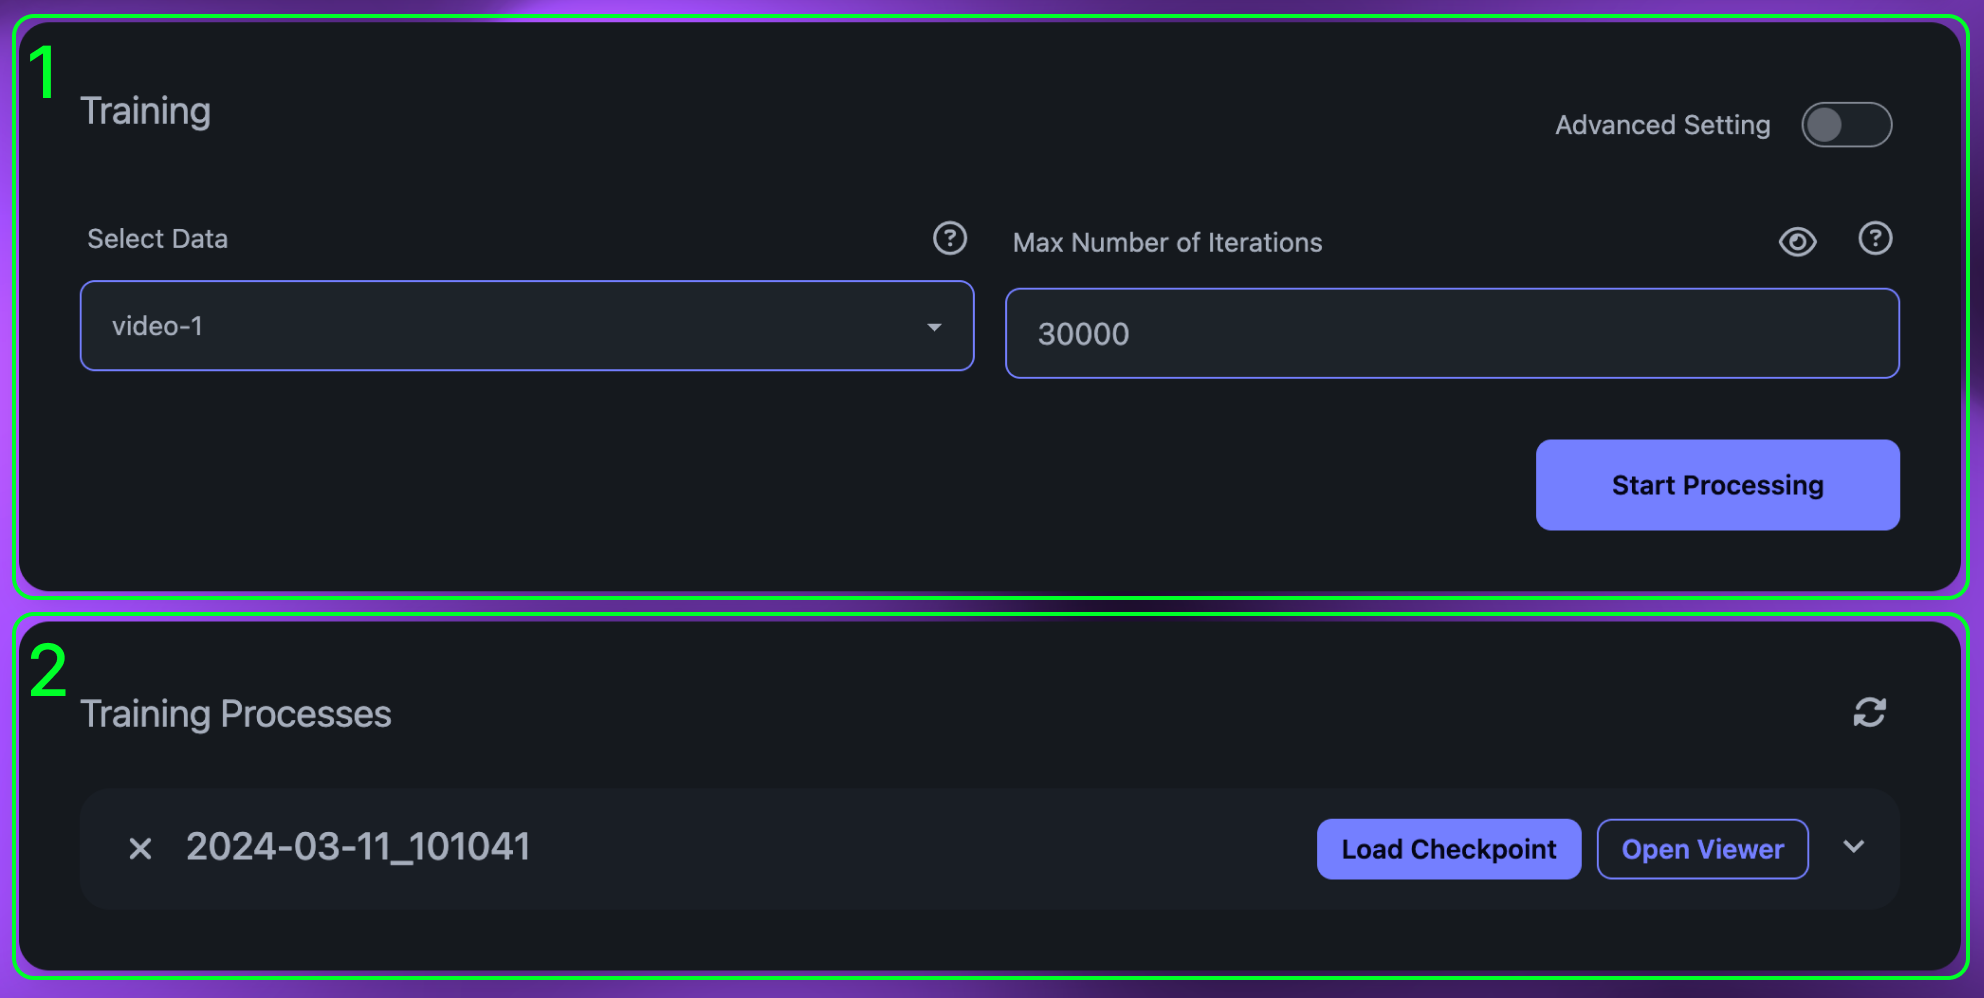
\includegraphics[width=\textwidth]{figures/view-train.png}
  \caption{Training Section}
  \label{fig:design:training-section}
\end{figure}

\subsubsection{Rendering Section}

The rendering section is the final step in the process, and allows users to render the final NeRF model.
At its core is the Nerfstudio Viewer that is integrated into the application. 
It provides users with all the functionality available in the standalone version, with a few integration that simplify the render process.
Instead of providing commands that have to be executed in the terminal, the rendering is started by clicking a button.

\begin{figure}[htb]
  \includegraphics[width=\textwidth]{figures/view-viewer.png}
  \caption{Viewer Section}
  \label{fig:design:viewer-section}
\end{figure}